\subsection{Oblate spheroidal fluid particles}


% \subsubsection{Shape description of the droplet}
We now consider that all particles possess an oblate spheroidal shape as represented in \ref{fig:scheme_spheroid}. 
This shape is advantageous because, for small deformations, it has been theoretically shown that droplets and bubbles tend to adopt an ellipsoidal shape. 
This holds for particles undergoing sedimentation \citep{taylor1964deformation}. 
For droplets immersed in pure linear flows it is shown that, in the limit of small deformation, the droplet shape also remain spheroidal \citep{leal2007advanced}. 
However, droplets immersed in quadratic flows do not deform as ellipsoids, as shown by \citet{nadim1991motion}. 
This implies that, for instance, in the closure problem, we must neglect the quadratic contributions from the carrier fluid. 
\begin{figure}[h!]
    \centering
    \hfill
    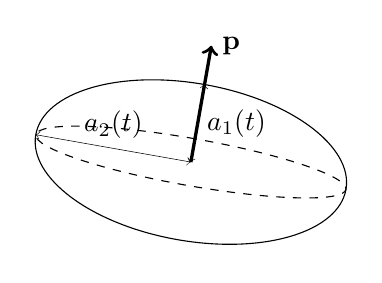
\begin{tikzpicture}[rotate=80]
        \draw(0,0) ellipse (1 cm and 2 cm);
        \draw[dashed](0,0) ellipse (0.3 cm and 2 cm);
        \draw[<->,very thin](0,0) --++ (1,0)node[midway,right]{$a_1(t)$};
        \draw[->,very thick](0,0) --++ (1.5,0)node[right]{$\textbf{p}$};
        \draw[<->,very thin](0,0) --++ (0,2)node[midway,above]{$a_2(t)$};
    \end{tikzpicture}
    \hfill
    \caption{Scheme of an  oblate spheroid oriented along the unit vector \textbf{p} with $a_f(t)$ and $a_2(t)$ the length of the semi axes of the spheroid.
    Note that when the drop is spherical we have $a_f=a_2=a$}
    \label{fig:scheme_spheroid}
\end{figure}

The shape of a particle is entirely described by an orientation vector $\textbf{p}$ and its two semi-axis, $a_1$ and $a_2$.  
By direct integration over the spheroidal particle volume in its local reference frame, i.e. the reference frame formed by $\textbf{p}$ and two other orthogonal unit vectors, it can be shown that $M_1$ and $M_2$ which are the eigenvalues of $\textbf{M}_\alpha$, read as,
\begin{align*}
    M_1 = \frac{m_\alpha a_1^2}{5},
    && M_2 = \frac{m_\alpha a_2^2}{5}.
\end{align*}
Since the particle volume remains constant over time, as given by  \ref{eq:dt_m_alpha}, we can state that $a_2^2 a_1 =a^3$, where $a$ is the radius of the equivalent spherical particle.
To measure the deviation from a spherical shape, we use the dimensionless properties $\chi_I$ and $\chi_{II}$ defined as, $\chi_I = (a_1/a)^2 - 1$ and $\chi_{II} = (a_2/a)^2 - 1$. 
With this definition, $\chi_I = 0$ when, $a_1/a =1$, in other worlds $\chi_I =\chi_{II} = 0$ when the droplet is spherical. 
Thus, $\chi_I$ will be termed the first aspect ratio of the droplet.  
Based on these definitions, the volume conservation condition \eqref{eq:dt_m_alpha} implies that $\chi_{II} = (\chi_I + 1)^{-1/2} - 1$.
% $a_2^2 a_1 =a^3 \to \chi_{II} + 1 = a /a_1$
% $\chi_I = (a_1/a)^2 - 1 \to (\chi_I +1)^{-1/2} = a/a_1$
% $a_1/a = a^2/a_2^2$
% Thus, the droplets shape is entirely determined by its orientation vector and one of its aspect ratio $\chi_I = a_1/a$ or $\chi_{II} = a_2^2/a^2$. 
Considering all these remarks we may describe the droplet shape using the dimensionless tensor, 
\begin{equation*}
    \bm\chi_\alpha
    = \frac{5}{m_\alpha a^2}\textbf{M}_\alpha - \bm\delta
    = \chi_I \textbf{pp}
        +[(\chi_I + 1)^{-1/2} - 1 ] (\bm\delta - \textbf{pp}). 
\end{equation*}
Thus, the droplet spheroidal shape is entirely characterized by two relevant parameters: the orientation vector \textbf{p} and its aspect ratio $\chi_I$.
It is interesting to note that since $\textbf{p}$ is an eigenvector of $\textbf{M}_\alpha$ and $\bm\chi_\alpha$, $\chi_I$ and $\chi_{II}$ constitute the eigenvalues of $\bm\chi_\alpha$. 
Additionally, note that with the definition used here, $\bm\chi_\alpha +\bm\delta$ corresponds to the Cauchy green deformation tensor often employed in solid mechanics \citep{mwasame2018macroscopic}. 
The geometrical description of the surface of the droplet can also be obtained using the tensor $\bm\chi_\alpha$. 
Indeed, the distance function  $f_\alpha(\textbf{x})$, describing the particle ellipsoidal surface can be defined as \citep{nadim1996concise},  
\begin{equation*}
    f_\alpha(\textbf{x}_\alpha +\textbf{r},t) = \textbf{rr}:(\bm\chi_\alpha +\bm\delta)-a^2.  
    \label{eq:distance_function}
\end{equation*}
It is to be understood from this definition that the points $\textbf{x}$ lying on the surface of the particles respect the constraint $f_\alpha(\textbf{x},t) = 0$. 
Being able to define the droplet's surface in this way will find its use in the calculation of the surface tension stress term present in \ref{eq:dt_S_alpha}. 

% \begin{remark}{Hypothesis of small deformation :}
    
% \end{remark}
\paragraph*{Hypothesis of small deformation: }
A droplet in a pure linear flow will deform into an spheroidal shape \citet{leal2007advanced} at first order in capillary number. 
A buoyant rising droplet with the effect of small inertia will deform at the first order in $Re$ into an ellipsoid as well \citep{taylor1964deformation}.
However, as soon as the inertial effects become higher or the flow quadratic for example, the droplets' deformation is found to exhibit other shapes than spheroidal \citep{taylor1964deformation,stone1990simple}.
Therefore, in this work, we limit our study to small deformations since as soon as the droplet deformation reaches high values one might expect other shapes than ellipsoid, which is in contradiction with the initial assumption. 
Thus, to stay within our study's hypothesis we may consider only small deformation. 
This means that we neglect all the term of $\mathcal{O}(\chi_I^2)$ or $\mathcal{O}(\chi_{II}^2)$ or higher. 
In this situation note that $\chi_{II} = (\chi_I + 1)^{-1/2} -1 \approx  - \chi_I /2$. 
Thus, the deformation tensor can be written in the simple form, 
\begin{equation}
    \bm\chi 
    = \chi_I
    \left[
        \textbf{pp} 
        - \frac{1}{2}(\bm\delta - \textbf{pp})
    \right]
    = \chi_I \frac{1}{2} \left[
        3 \textbf{pp} - \bm\delta
    \right]
    \label{eq:chi_I_small_def}
\end{equation}
Thus, the trace of $\bm\chi_\alpha$ may be written for small deformation as :  $\bm\delta:\bm\chi_\alpha  = \chi_I + 2\chi_{II} = \mathcal{O}(\chi_{I}^2)$, in other worlds for small deformation $\bm\chi_\alpha$ is purely deviatoric. 
Thus, the trace of $\bm\chi_\alpha$ is null only when considering small deformations. 
This property will be useful in the following sections.
Note that at the next order of deformation, we have $\bm\delta:\bm\chi_\alpha  = \chi_I + 2\chi_{II} = 3 \chi_I^2 /4 +  \mathcal{O}(\chi_{I}^3)$. 

\subsection{Droplet internal velocity field}

Now that the droplet shape is properly defined we turn our attention to the description of the internal flow present within the droplets.
Indeed, the droplet internal flow $\textbf{w}_d^0$ present in the closure terms of \ref{eq:dt_S_alpha} is not part of the Lagrangian unknown, and therefore must be either directly closed or related to the Lagrangian properties which are part of the unknown of the problem.  
In \citet{lhuillier1987phenomenology} he assumes that the flow within the droplets is linear with the position. 
In our notation, this means that $\textbf{w}_d^0 = \textbf{r}\cdot \textbf{E}_\alpha(t)$ where $\textbf{E}_\alpha(t)$ corresponds to the mean rate of strain of the particle. 
In this case, $\textbf{E}_\alpha(t)$ constitutes an unknown of the particle phase which is solved in \citet{lhuillier1987phenomenology} with an equation similar to \ref{eq:dt_S_alpha}. 
For deformable solid bodies, this approach is accurate since the internal velocity field is indeed linear.
Nevertheless, as discussed in \citet{lhuillier1987phenomenology} for fluid droplets, the internal velocity field $\textbf{w}_d^0$ is far from being linear, as $\textbf{w}_d^0$ exhibits complicated fluid circulation in most of the situations, and this hypothesis is somewhat doubtful. 
Consequently, in this work, we adopt a more general approach that still accounts for the complicated internal flow present inside the particles while using a mean rate of strain tensor, $\textbf{E}_\alpha(t)$, to account for the linear deforming motions. 

It is known that an isolated droplet in creeping flow condition with relative translating motion with the carrier fluid exhibits internal motions. In this specific situation the streamlines formed by $\textbf{w}_d^0$ are known as Hill vortices, see \ref{fig:flowlines1} (b).
In this case $\textbf{w}_d^0$ has a term proportional to \textbf{rr}.  
If slightly more inertial effects are present, the initially spherical droplet deforms into an oblate spheroid \citep{taylor1964deformation}, and one might find that the internal motion of such a spheroid is close to Hill vortexes but with an oblate spheroidal shape, see \ref{fig:flowlines1} (c). 
For a drop immersed in an unbounded pure linear flow, still in stokes flow, we can derive an analytical solution for $\textbf{w}_d^0$ and find that $\textbf{w}_d^0 \sim \textbf{rrr}$ with $\textbf{r}$ the position in space relative to the center of mass of the particle, see \ref{fig:flowlines1} (a), (see \ref{chap:closure-disperse}). 
Thus, in all those cases the internal motions are more complicated than a simple linear velocity field since the internal flow is rather quadratic or cubic. 
Moreover, in all those cases the droplet's internal velocity fields are steady-state solutions.
However, for a droplet to transition from the state depicted in \ref{fig:flowlines1} (b) to the state shown in \ref{fig:flowlines1} (c) it must deform from a sphere to an oblate ellipsoid. 
Equally, a droplet immersed in a pure linear flow may experience deformation, in that case, $\textbf{w}_d^0$ and the shape of the droplet may be a function of time and capillary number \citet[chapter 7]{leal2007advanced}.
\begin{figure*}
    \centering
    \begin{tikzpicture}
        \node (img3) at (0.6\textwidth,0) {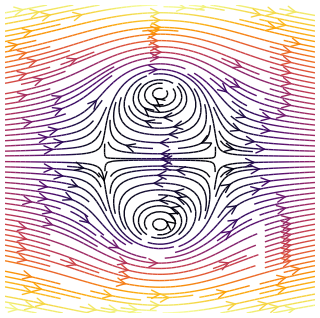
\includegraphics[width=0.3\textwidth,angle=270]{image/Rising_def_Stokes.png}};
        \node (img2) at (0.3\textwidth,0) {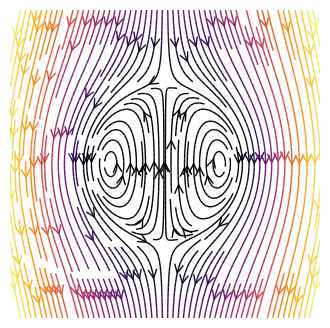
\includegraphics[width=0.3\textwidth]{image/Rising_Stokes.png}};
        % \draw (0.45\textwidth,0)node{$\rightarrow$};
        % \draw (0.45\textwidth,0.4cm)node{$\bm\Gamma_\alpha\cdot \textbf{r}$};
        \node (img1) at (0.0\textwidth,0) {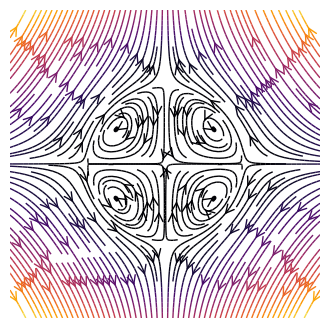
\includegraphics[width=0.3\textwidth]{image/Shear_Stokes.png}};
        \draw (img3.south)node{(c)};
        \draw (img2.south)node{(b)};
        \draw (img1.south)node{(a)};
    \end{tikzpicture}
    \caption{Three examples of steady state flow lines plots of an isolated droplet immersed into a viscous fluid. 
    (a) Fixed droplet in extensional flow (analytical solution in \ref{chap:daniel2}).
    (b) Rising sphere in uniform stokes flow (analytical solution in \ref{chap:daniel2}). 
    (c) Deformed droplet in rising motion (analytical solution of \citet{taylor1964deformation}). }
    \label{fig:flowlines1}
\end{figure*} 

To account for this deformation in our case we assume that the \textit{transient internal velocity field} which is responsible for this deformation is homogeneous and linear with position \textbf{r}. 
Thus, the \textit{transient internal velocity field} of a particle can be modeled as $\textbf{w}_d^0 = \bm\Gamma_\alpha \cdot \textbf{r}$, where we have introduced, $\bm\Gamma_\alpha$, the mean velocity gradient inside the particle, which symmetric part: $\textbf{E}_\alpha$, represents the rate of strain, and skew-symmetric part: $\bm\Omega_\alpha$, represents the angular velocity. 
Note that the angular velocity tensor $\bm\Omega_\alpha$ is related to the angular velocity \textit{pseudo} vector $\bm\omega_\alpha$ with the relation $\bm\omega_\alpha = -\frac{1}{2}\epsilon_{ijk} (\bm\Omega_\alpha)_{jk}$. 
To summarize, we assume that the inner velocity field of the drop can be decomposed into two distinct parts. 
The first one is the steady-state component, examples are: Hill's vortices for a spherical drop in uniform linear motion, the Hill vortices-like velocity field observed for oblate spheroidal droplets in translation,  the inner velocity field of a drop in steady-state linear flows, and so on.  
The second contribution is the inner velocity fields that alter the drop's shape, this field is assumed linear with the position and homogeneous, it reads  $\bm\Gamma_\alpha\cdot \textbf{r}$. 
Adopting these definitions, the particle's internal velocity is decomposed as, 
\begin{equation}
    \textbf{w}_{d}^0[\textbf{x}_\alpha(t)+\textbf{r},t]
    = \bm\Gamma_{\alpha} \cdot \textbf{r}
    + \textbf{v}^0_{d}[\textbf{r},t]
    =\bm{\Omega}_{\alpha}\cdot \textbf{r}
    + \textbf{E}_{\alpha} \cdot \textbf{r}
    + \textbf{v}^0_{d}[\textbf{r},t]
    \label{eq:def_vel}
\end{equation}
Where we introduced the vector $\textbf{v}^0_d[\textbf{r},t] =\textbf{w}^{0}_{d}[\textbf{x}_\alpha(t)+\textbf{r},t]  - \bm\Gamma_{\alpha}[t] \cdot \textbf{r}$.
With this definition $\textbf{v}_d^0$ represents the particle's internal motion that does not contribute to the linear homogeneous deformation and angular rotation of the drop. 
Thus, $\textbf{v}_d^0$ could be one of the three velocity fields presented in \ref{fig:flowlines1}. 

Due to the consideration of mass conservation \eqref{eq:dt_m_alpha} additional properties can be noted for the tensor $\textbf{E}_\alpha$.
Indeed, at steady-state the local mass conservation inside the particle imposes that $\div \textbf{v}_d^0 = 0$. 
Thus, for a deformable droplet we obtain that $\div \textbf{u}_d^0 = \bm\Gamma_\alpha : \bm\delta = \textbf{E}_\alpha : \bm\delta =  0$.  
Also, note that to preserve the spheroidal shape of the particle we must assume that the particle's rate of strain principal direction is the same as the droplet's shape principal axis. 
In other words, $\textbf{E}_\alpha$ must have the same eigenbasis as $\textbf{M}_\alpha$. 
Making up with these two constrain leads to the expression: $\textbf{E}_\alpha = E_I \textbf{pp} + E_{II} (\bm\delta - \textbf{pp})$, where $E_I$ and $E_{II}$ are the first and second eigenvalue of $\textbf{E}_\alpha$ which are related through $E_I = - 2E_{II}$ due to the volume conservation constraint, ($\bm\delta : \textbf{E}_\alpha =0$). 


Let us now introduce the upper-convected time derivative, also known as the Oldroyd derivative, for an arbitrary Lagrangian second-order tensor $\textbf{A}$ with respect to the mean gradient $\bm\Gamma_\alpha$. 
This derivative is expressed as: 
\begin{equation}
    \overset{\triangledown  }{\textbf{A}}
    = 
    \ddt \textbf{A}
    - \textbf{A} \cdot \bm\Gamma_\alpha
    - \bm\Gamma_\alpha \cdot \textbf{A}
    \label{eq:def_upper}
\end{equation}
The physical interpretation of this operator is that it represents the time derivative of the tensor $\textbf{A}$ in a coordinate system rotating and stretching according to $\bm\Gamma_\alpha$.  
According to our assumption, the droplet shape $\textbf{M}_\alpha$ remains spheroidal under the linear transformation governed by $\bm\Gamma_\alpha$, it is self-similar. 
Additionally, recall that the field $\textbf{r}\cdot \bm\Gamma_\alpha$ accounts for the entire deformation of the droplet. 
Consequently, we deduce that:
\begin{equation}
    \overset{ \triangledown  }{\textbf{M}}_\alpha
    = 0, 
    \label{eq:def_conseq}
\end{equation}
since the shape of the droplet seen in a coordinate system that stretches and rotates with $\bm\Gamma_\alpha$ does not change \footnote{
    This expression is analogous to the definition used in rheology, which states that the upper-convected time derivative of the Finger tensor is always zero.
}.
On the other hand, substituting $\textbf{w}_d^0$ by its definition \eqref{eq:def_vel} in \ref{eq:dt_M_alpha}, gives, 
\begin{equation}
    \ddt \textbf{M}_{\alpha,ik}
    -
    \textbf{M}_{\alpha,ik} \cdot \bm\Gamma_{\alpha,kj}
    -  \bm\Gamma_{\alpha,ki} \cdot \textbf{M}_{\alpha,jk}
    =
    \intO{ 
        (\textbf{v}_{d,i}^0\textbf{r}_j
        + \textbf{r}_i\textbf{v}_{d,j}^0)
    },
\end{equation}
where we have used the Einstein indices summation convention. 
Using the definition of the upper-convected derivative given by \ref{eq:def_conseq}, leads us to the relation,
\begin{equation}
    % \overset{ \footnotesize \triangledown  }{\textbf{M}}_\alpha
    % = 
    \intO{ 
        (\textbf{v}_{d,i}^0\textbf{r}_j
        + \textbf{r}_i\textbf{v}_{d,j}^0)
    }
    =
    0.  
    \label{eq:def_v}
\end{equation}
In summary, the assumption that the droplet shape remains spheroidal and that only the linear velocity field $\textbf{r}\cdot \bm\Gamma_\alpha$ were responsible for the droplet deformation, leads us to the conclusion that $\overset{\triangledown}{\textbf{M}}_\alpha= 0$. 
Then, using the evolution equation for $\textbf{M}_\alpha$ leads us to \ref{eq:def_v}, which can be interpreted as a constraint that the field $\textbf{v}_d^0$ must satisfy. 
Thus, $\textbf{v}_d^0$ is defined by the general relation $\textbf{v}^0_d[\textbf{r},t] =\textbf{w}^{0}_{d}[\textbf{x}_\alpha(t)+\textbf{r},t]  - \bm\Gamma_{\alpha}[t] \cdot \textbf{r}$ and the constraint given by \ref{eq:def_v}. 
One can remark that this constraint is satisfied by each of the solutions represented in \ref{fig:flowlines1}.
This can be verified for the case (a) and (b) with the analytical solution provided in \ref{chap:closure-disperse}. 



% Likewise, $\textbf{v}_d^0$ is assumed not to affect the particle's angular momentum, as the kinematics   description of the angular momentum is solely based on its angular velocity $\bm\Omega_\alpha$, just as $\textbf{E}_\alpha$ is assumed to be the only source of deformation. 
% The kinematics   description of the angular momentum relies solely on the particle's angular velocity.
% This assumption means that the velocity decomposition has the desirable property that: $\textbf{P}_\alpha = \bm\Gamma_\alpha \cdot \textbf{M}_\alpha + \intO{\textbf{v}^0_{d,i} \textbf{r}_j} =  \bm\Gamma_\alpha \cdot \textbf{M}_\alpha $, at all times, since $\textbf{v}^0_{d,i} $ is not supposed to contribute to either the angular momentum or the symmetric part of the momentum. 
% As it will be shown this simplifies the equations of motion without entirely neglecting the internal motion.
% This means that $\textbf{v}^0_{d}$ can depend on the current shape of the particle through $\textbf{M}_\alpha$ or $\bm\chi_\alpha$ (as shown in \ref{fig:flowlines1} (c)) or its current center of mass velocity $\textbf{u}_\alpha$ (since the Magnitude of Hill vortex depends on the particle center of mass velocity), however, it must satisfy the condition $\intO{\textbf{v}^0_{d,i} \textbf{r}_j}  = 0$.



As demonstrated in \ref{chap:closure-disperse} the internal motions of an isolated spherical drop, such as the one presented in  \ref{fig:flowlines1}, are entirely determined  from $\textbf{u}_f$,$\grad\textbf{u}_f$ and $\textbf{u}_\alpha$ and the shape of the particle. 
Therefore, it is reasonable to assume that in a more general case, $\textbf{v}_d^0$ might be entirely determined by the carrier fluid and particles' properties, specifically, $\textbf{u}_\alpha$ $\textbf{M}_\alpha$, $\textbf{u}_f$ and $\grad\textbf{u}_f$. 
For non-dilute flows we might even, need to consider the volume fraction $\phi_d$ or more complicated functions.
However, this chapter will not delve into these considerations and will focus solely on dilute scenarios.
From now on we consider that the internal velocity $\textbf{v}^0_d(t,\textbf{r})$ is not part of the particle' unknown, but rather as a closure term that should be expressed in terms of $\textbf{u}_\alpha$ $\textbf{M}_\alpha$, $\textbf{u}_f$ and $\grad\textbf{u}_f$. 
Consequently, in this problem, we will explore and demonstrate how a single droplet can be exhaustively described by the parameters, $\textbf{x}_\alpha, \textbf{u}_\alpha, \bm\chi_\alpha$ and $\bm\Gamma_\alpha$, while accounting for more complex internal motion inside the droplets through different closure terms.
As we have seen $\bm\chi_\alpha$ and $\bm\Gamma_\alpha$ may also be replaced by the scalars $\chi_I$, $E_I$ and the vector \textbf{p} and $\bm\omega_\alpha$. 

\subsection{Conservation equations}

Now that the particle's shape and internal kinematics   are properly defined we may simplify the moments of mass and momentum equations. 
The integrals appearing in \ref{eq:dt_M_alpha}, \ref{eq:dt_mu_alpha} and \ref{eq:dt_S_alpha} can be reformulated using the definition of $\textbf{w}_d^0$ adopted in \ref{eq:def_vel}, to find, 
\begin{align}
    \textbf{M}_\alpha 
    = \intO{ \rho_d \textbf{rr} }
    = \frac{m_\alpha a^2}{5} (\bm\chi_\alpha+\bm\delta)\\
    % \textbf{P}_\alpha = \textbf{M}_{\alpha,ik} \cdot \bm\Gamma_{\alpha,jk}\\
    \bm\mu_\alpha 
    = \intO{ \rho_d \textbf{r}\times\textbf{u}_d^0 }
    = \textbf{I}_\alpha \cdot \bm\omega_\alpha
    + \intO{ \rho_d \textbf{r}\times\textbf{v}_d^0 }
    \\
    \label{eq:S_def}
    \textbf{S}_{\alpha,ij} = \intO{(\textbf{rw}_ 2^0 )_{ij}+ (\textbf{w}_d^0 \textbf{r})_{ij}} 
    = \textbf{M}_{\alpha,ik} \cdot \bm\Gamma_{\alpha,jk}
        +  \bm\Gamma_{\alpha,ik} \cdot \textbf{M}_{\alpha,jk}
    \\
    \intO{\rho_d \textbf{v}_{d,i}^0\textbf{v}_{d,j}^0}
    = \bm\Gamma_{\alpha,jl}\bm\Gamma_{\alpha,ik} \textbf{M}_{\alpha,kl}  
    +\intO{\rho_d \textbf{v}_{d,i}^0\textbf{v}_{d,j}^0}
    \label{eq:ww_def}
    \\
    \label{eq:sigma_d_def}
    \intO{\bm\sigma_{d,ij}^0}
    =
    2 \mu_d v_\alpha \textbf{E}_{\alpha,ij}
    - \intO{p_d^0} \bm\delta_{ij}
    + \mu_d \intS{(\textbf{n}_i \textbf{v}_{d,j}^0 + \textbf{n}_j \textbf{v}_{d,i}^0)}
    \\
    \intS{\bm\sigma_{I,ij}^0}
    = \frac{\gamma v_\alpha }{a} \left[
        2\bm\delta_{ij} 
        + \frac{4  }{5} \bm\chi_{\alpha,ij}
    \right]
    +\mathcal{O}(|\bm\chi_\alpha|^2)
    % s_\alpha 
    % = 4\pi a^2 (1+\frac{\textbf{M}:\textbf{M}}{15})
\end{align}
where we have introduced the \textit{inertia moment} of the particle $\alpha$ as $\textbf{I}_\alpha = (\bm\delta : \textbf{M}_\alpha)\bm\delta - \textbf{M}_\alpha$. 
These expressions are rather straightforward since one only needs to use the definition of $\textbf{w}_d^0$ in these integrals. 
However, the surface tension stress tensor, $\intS{\bm\sigma_{I,ij}^0}$, is not so easy to obtain since it requires carrying an integral over the spheroidal surface of the particle.
Thus, the detailed calculation of the surface tension stress tensor is given in \ref{ap:surface_tension}. 
We provide the exact results as well as the Taylor expansion of this formula for small deformation. 
Note that the spheroidal shape remains valid only for small deformations; therefore, the exact formula for $\intS{\bm\sigma_{I,ij}^0}$ considering arbitrary deformation is of limited interest. 
It is good to note that our formula agrees with the one derived by \citet{lhuillier1987phenomenology} but with the addition of the higher order term not present in this study. 
Additionally, we can observe that two new integrals terms appeared on the right-hand side of \ref{eq:sigma_d_def}  and \ref{eq:ww_def}. 
They correspond respectively to the particle internal viscous stress and the particle internal inertial motions generated by $\textbf{v}_d^0$.
As discussed in the preceding subsection, these contributions arise from motions that are independent of particle deformation and rotation and must be treated as closure terms. 



Injecting these formulas inside \ref{eq:dt_M_alpha}, \ref{eq:dt_mu_alpha}, \ref{eq:dt_S_alpha} yields an equation for $\bm\chi_\alpha$, $\bm\omega_\alpha$ and $\textbf{E}_\alpha$, namely,
\begin{align}
    % \ddt \textbf{pp}_{\alpha,ij}
    % = \textbf{pp}_{\alpha,ik} \cdot \bm\Omega_{\alpha,jk}
    % +  \bm\Omega_{\alpha,ik} \cdot \textbf{pp}_{\alpha,jk}\\
    \overset{ \triangledown  }{\bm\chi}_\alpha
    = 
    \ddt \bm\chi_{\alpha,ij}
    -\bm\chi_{\alpha,ik} \cdot \bm\Gamma_{\alpha,jk}
    - \bm\Gamma_{\alpha,ik} \cdot \bm\chi_{\alpha,jk}
    =
    2\textbf{E}_{\alpha,ij},
    \label{eq:dt_M2}
    \\
    \ddt (\textbf{I}_{\alpha,ik}\bm\omega_{\alpha,k} )
    = 
    \intS{(\textbf{r}\times\bm\sigma_f^0\cdot \textbf{n})_i}
    - \ddt\intO{\rho_d(\textbf{r}\times \textbf{v}_d^0)_i},
    \label{eq:dt_mu2}
    \\
    \ddt \textbf{S}_{\alpha,ij}
    -  \bm\Gamma_{\alpha,jl}\bm\Gamma_{\alpha,ik} \textbf{M}_{\alpha,kl}  
    + \mu_d v_\alpha 2\textbf{E}_{\alpha,ij}
    + \frac{\gamma v_\alpha }{a} \left(
    2\bm\delta_{ij} 
    + \frac{4 }{5} \bm\chi_{\alpha,ij}
    \right) \nonumber\\
    = 
    \frac{1}{2}\intS{(\textbf{r}\bm\sigma_f^0 + \bm\sigma_f^0\textbf{r})_{ijk}\cdot \textbf{n}_k} 
    + \intO{\rho_d \textbf{v}_{d,i}^0\textbf{v}_{d,j}^0}
    + \bm\delta_{ij}\intO{p_d^0} \nonumber\\
    - \mu_d \intS{(\textbf{n}_i \textbf{v}_{d,j}^0 + \textbf{n}_j \textbf{v}_{d,i}^0)},
    \label{eq:dt_S2}
\end{align}
respectively. 
The second moment of mass \ref{eq:dt_M2}, represents the kinematics   equation describing the evolution of $\bm\chi_\alpha$ due to the particle elongation and rotation. 
Note that this expression is consistent with the equation obtained by \citet{goddard1967nonlinear} if one accounts for the slightly different definitions of $\bm\chi_\alpha$ and \textbf{C} in \citet{goddard1967nonlinear}.
Following \citet{goddard1967nonlinear} the left-hand side term of \ref{eq:dt_M2} is identified as the upper-convected derivative of $\bm\chi_\alpha$, which returns the rate of strain $\textbf{E}_\alpha$. 
The equation for the skew-symmetric part of the first moment of momentum \ref{eq:dt_mu2}, is the angular momentum balance of the particle when considering the moment of inertia of a deformable particle.
Note that in this expression the moment of inertia $\textbf{I}_\alpha$ arises naturally since its use simplifies the expression. 
The first term on the right-hand side of \ref{eq:dt_mu2} accounts for the hydrodynamic torque contribution due to the surrounding fluid.
And, the second term represents the changes of angular momentum generated by inner velocity currents. 
The symmetric part of the moment of momentum equations \ref{eq:dt_S2} is an equation for the rate of deformation, $\textbf{E}_\alpha$. 
The first two terms on the left-hand side correspond to the inertial contribution of the mean droplet rate of deformation $\textbf{E}_\alpha$. 
The third term corresponds to the contribution of the droplet's internal stress generated due to the mean drop deformation. 
The last term on the left-hand side is the contribution from the surface tension force which is the only reason why the droplet shape reaches a spherical shape equilibrium. 
These terms are directly related to either $\bm\chi_\alpha$, $\bm\omega_\alpha$ or $\textbf{E}_\alpha$, our unknowns, therefore they are gathered on the left-hand side of the equation. 
On the right-hand side of the equation, we gathered every forcing term, or closure term that is not explicitly a function of the droplet's current shape or deformation.  
The first term is the first moment of the external hydrodynamic forces, $\intS{(\textbf{r}\bm\sigma_f^0+ \bm\sigma_f^0\textbf{r})\cdot \textbf{n}}$ which is a function of the external flow properties but also of the current droplet properties. 
The second forcing term comes from the internal droplet inertia, that is the inertia related to the internal circulation of the drop. 
The third term is the mean droplet's hydrostatic pressure which is balanced mainly by the isotropic part of the surface tension contribution and the mean fluid pressure. 
The last term on the right-hand side then corresponds to the internal viscous stress generated by the relative motion of the drop with the carrier fluid. 


From \ref{eq:dt_D_alpha} we can also derive a conservation for the trace of $\bm\Gamma_\alpha$ which reads, 
\begin{equation}
    -  \bm\Gamma_{\alpha,ml}\bm\Gamma_{\alpha,mk} \textbf{M}_{\alpha,kl}  
    + \frac{\gamma v_\alpha }{a} 
    \left[
    2\bm\delta_{mm} 
    % - \frac{4 }{5 } (\textbf{M}_{\alpha,mm}^* - \textbf{I}_{\alpha,mm})
    \right]
    = 
    \intS{\textbf{r}_m\cdot\bm\sigma_{f,mk}^0\cdot \textbf{n}_k} 
    + \intO{\rho_d \textbf{v}_{d,m}^0\cdot \textbf{v}_{d,m}^0}
    + \intO{p_d^0} \bm\delta_{mm},
    \label{eq:dt_trM2}
\end{equation}
This equation, corresponds to a scalar equation describing the dynamical balance of the isotropic part of the moment of momentum of the particle. 
This equation contains the trace of every term present in \ref{eq:dt_S2} except that both viscous terms and the derivative of the trace of $\textbf{S}_\alpha$ canceled since they are traceless tensors. 
Note that the second term on the left-hand side is the isotropic part of the surface tension forces, it corresponds to the well-known Laplace pressure. 
Additionally, on the right-hand side of \ref{eq:dt_trM2} we note the trace of the hydrodynamic forces, which together with the particle internal pressure form the Laplace equation. 
Nevertheless, \ref{eq:dt_trM2} is more general than the classic Laplace equilibrium equation as it includes inertial effects as well as particle internal motions and deformations effects.  
Initially, \ref{eq:dt_trM2} is supposed to be used as an equation for $M_\alpha$, or more precisely the trace of $\bm\chi_\alpha$.
However, since the particle volume is assumed constant, \ref{eq:dt_trM2} can be considered as an equation for the particle mean internal pressure. 
Indeed, using that expression to cancel out the particle pressure in \ref{eq:dt_S2} gives us a novel expression that describes the deviatoric part of $\textbf{M}_\alpha$ or $\bm\chi_\alpha$.
Therefore, it corresponds to the description of the deviation from the spherical particle's shape $\bm\chi_{\alpha,ij}$. 
Indeed, injecting \ref{eq:dt_trM2,eq:dt_M2,eq:S_def} into  \ref{eq:dt_S2} one obtain, 
\begin{align}
        \ddt^2 \bm\chi_{\alpha,ij}
        - 2(\bm\chi_{\alpha,kl} + \bm\delta_{kl})
        (\bm\Gamma_{\alpha,jl}\bm\Gamma_{\alpha,ik}  
        - \frac{1}{3}
        \bm\Gamma_{\alpha,ml}\bm\Gamma_{\alpha,mk}  
        \bm\delta_{ij}
        )
    &+ 
    \frac{1}{\tau_\mu}
    \overset{ \triangledown  }{\bm\chi}_\alpha
    +
    \frac{1}{\tau_\gamma^2}
    \bm\chi_{\alpha,ij}
    = 
    10 \textbf{F}_{ij}
    \label{eq:dev}
\end{align}
where,
\begin{align}
    1/\tau_\mu 
    =
    \frac{\mu_d 10}{\rho_d a^2}  
    &&
    1/\tau_\gamma^2
    = 
    \frac{\gamma 8 }{\rho_d a^3} 
\end{align}
and,
\begin{align}
    \textbf{F}_{ij}
    &= 
    \textbf{F}_{ij}^h
    +\textbf{F}_{ij}^{vv}
    + \textbf{F}_{ij}^{\sigma}\\
    \textbf{F}_{ij}^h
    &= \frac{1}{2m_\alpha a^2}\intS{(\textbf{r}\bm\sigma_f^0 + \bm\sigma_f^0\textbf{r} - \frac{2}{3}(\textbf{r}\cdot \bm\sigma_f^0) \bm\delta)\cdot \textbf{n}} \\
    \textbf{F}_{ij}^{vv}
    &= 
    \frac{1}{m_\alpha a^2}\intO{\rho_d(\textbf{v}_{d,i}^0\textbf{v}_{d,j}^0 - \frac{1}{3}\textbf{v}_{d,m}^0\textbf{v}_{d,m}^0 \bm\delta_{ij}) }\\
    \textbf{F}_{ij}^{\sigma}
    &= - \frac{\mu_d}{m_\alpha a^2} \intS{(\textbf{n}_i \textbf{v}_{d,j}^0 + \textbf{n}_j \textbf{v}_{d,i}^0)}\nonumber
\end{align}
where we have gathered all the closures or forcing terms into the tensor $\textbf{F}_{ij}$ which has the unit [s$^{-2}$]. 
% Note that $\textbf{E}_{\alpha,ij}$ is related to the \textit{convected} derivative of $\bm\chi_\alpha$ through \ref{eq:dt_M2}. 
One might recognize in \ref{eq:dev} a forced second-order oscillatory harmonic equation.
Indeed, the left-hand side terms correspond to the second, first and zeroth order derivative of $\bm\chi$ (i.e. $\ddt^2 \bm\chi_{\alpha,}$, $\overset{ \triangledown  }{\bm\chi}_\alpha$ and $\bm\chi_\alpha$ respectively), with the addition of the non-linear term, $ (\bm\chi_{\alpha,kl}+\bm\delta_{kl}) 
(\bm\Gamma_{\alpha,jl}\bm\Gamma_{\alpha,ik}  
- \frac{1}{3}
\bm\Gamma_{\alpha,ml}\bm\Gamma_{\alpha,mk}  
\bm\delta_{ij}
)$, while the right-hand side terms correspond to the forcing terms. 

Although oscillatory harmonic equations are typically scalar, this formulation is more general and holds for the deformation tensor. 
Notably, the coefficients $\tau_\mu$ and $\tau_\gamma$ in \ref{eq:dev} which appear in front of $\overset{ \triangledown  }{\bm\chi}_\alpha$ and $\bm\chi_\alpha$ respectively, correspond precisely to the damping ratio and the natural time of the secondary mode of oscillation for nearly spherical droplets, as described by \citep{lamb1924hydrodynamics}. 
Indeed, in the case of freely oscillating droplets, the natural time governing the period of oscillation of droplet deformation is given by $\tau_\gamma = \sqrt{\frac{a^3\rho_d}{8 \gamma }}$ \citep{lamb1924hydrodynamics}. 
Likewise, the damping coefficient, which corresponds to the timescale over which oscillations decay, is given by  $\tau_\mu = a^2\rho_d/10 \mu_d$ \citep{lamb1924hydrodynamics}. 


To conclude, the system of equations formed by \ref{eq:dt_M2}, \ref{eq:dt_mu2} and \ref{eq:dev}, with unknown $\bm\chi_\alpha$, $\textbf{E}_\alpha$ and $\bm\omega_\alpha$, allows us to describe the deformation and the rate of deformation of a spheroidal droplet with constant volume.

\subsection{The dimensionless equations}


To enhance the physical understanding of \ref{eq:dev} we derive in the present section the dimensionless form of this equation. 
We assume that the forcing terms introduced in \ref{eq:dev} are governed by a timescale independent of the droplet's natural timescale, denoted as $\tau_u$. 
This is because the external solicitation timescale is imposed by the ``background flow'' condition and thus is quite independent of the current droplet rate of deformation. 
For example, the term $\textbf{F}_{ij}^{vv}$ representing the kinetic energy of the internal droplet velocity, is mainly driven by the relative velocity between the droplet's center of mass and the background flow. 
In fact in \ref{chap:closure-disperse} we compute this term in the situation represented in \ref{fig:flowlines1} (b) and show that $ \textbf{F}^{vv}\sim (\textbf{u}_f - \textbf{u}_p)(\textbf{u}_f - \textbf{u}_p)$. 
Thus, in this case, the timescale of the forcing term is given by $\tau_u = a /(\textbf{u}_f - \textbf{u}_p)$ and $\textbf{F}^{vv}$ scale as $a^2/\tau_u^2$. 
If the ``background flow'' is linear for example,  or if it represents isotropic turbulence, the principle stays the same and $\tau_u$ will be related to the background flow timescale. 
Consequently, the forcing terms can be defined proportional to the scales: 
% \begin{align*}
%     \textbf{F}_{ij}^h
%     &= \frac{1}{2v_\alpha}\intS{(\textbf{r}\bm\sigma_f^0 + \bm\sigma_f^0\textbf{r} - \frac{2}{3}(\textbf{r}\cdot \bm\sigma_f^0) \bm\delta)\cdot \textbf{n}} 
%     \sim \mu_f  /\tau_u \\
%     \textbf{F}_{ij}^{vv}
%     &= \frac{\rho_d}{v_\alpha}
%     \intO{(\textbf{v}_{d,i}^0\textbf{v}_{d,j}^0 - \frac{1}{3}\textbf{v}_{d,m}^0\textbf{v}_{d,m}^0 \bm\delta_{ij}) }
%     \sim  \rho_d a^2  /\tau_u^2 \\
%     \textbf{F}_{ij}^{\sigma}
%     &= - \frac{\mu_d}{v_\alpha} \intS{(\textbf{n}_i \textbf{v}_{d,j}^0 + \textbf{n}_j \textbf{v}_{d,i}^0)}
%     \sim  \mu_d  /\tau_u. 
% \end{align*}
\begin{align}
    \textbf{F}_{ij}^h
    &= \frac{1}{2m_\alpha a^2}\intS{(\textbf{r}\bm\sigma_f^0 + \bm\sigma_f^0\textbf{r} - \frac{2}{3}(\textbf{r}\cdot \bm\sigma_f^0) \bm\delta)\cdot \textbf{n}} 
    \sim\mu_f  /(\tau_u \rho_d a^2)\\
    \textbf{F}_{ij}^{vv}
    &= 
    \frac{ \rho_d}{m_\alpha a^2}\intO{(\textbf{v}_{d,i}^0\textbf{v}_{d,j}^0 - \frac{1}{3}\textbf{v}_{d,m}^0\textbf{v}_{d,m}^0 \bm\delta_{ij}) }
    \sim 1/\tau_u^2\\
    \textbf{F}_{ij}^{\sigma}
    &= - \frac{  \mu_d}{m_\alpha a^2} \intS{(\textbf{n}_i \textbf{v}_{d,j}^0 + \textbf{n}_j \textbf{v}_{d,i}^0)}\sim 1 /(\rho_d  a^2  \tau_u^2)
\end{align}
Where it has been assumed that the term $\textbf{F}_{ij}^h$ scale as a viscous force. 
Multiplying \ref{eq:dt_trM2} by $\tau_\gamma^2$ and considering these scales yields the dimensionless tensor equation, 
\begin{multline}
    \tau_\gamma^2
    \left[
        \ddt^2 \bm\chi_{\alpha,ij}
        -  2 (\bm\chi_{\alpha,kl} + \bm\delta_{kl})
        (\bm\Gamma_{\alpha,jl}\bm\Gamma_{\alpha,ik}  
        - \frac{1}{3}
        \bm\Gamma_{\alpha,ml}\bm\Gamma_{\alpha,mk}  
        \bm\delta_{ij}
        )
    \right]\\
    + \frac{\tau_\gamma^2}{\tau_\mu} \overset{ \triangledown  }{\bm\chi}_\alpha
    + \bm\chi_{\alpha,ij}
    =\frac{5}{4} Ca [
    (\textbf{F}_{ij}^h )^*
    + \zeta Re (\textbf{F}_{ij}^{vv})^*
    + \lambda (\textbf{F}_{ij}^{\sigma})^*
    ] 
    \label{eq:dev_dim}
\end{multline}
where we have defined the following dimensionless groups : 
\begin{align*}
    \zeta = \rho_d /\rho_f,
    && \lambda = \mu_d/\mu_f,
    && Re = \frac{\rho_f a^2 }{ \mu_f \tau_u},
    && Ca = \frac{a \mu_f}{\gamma \tau_u}. 
\end{align*}
The superscript $^*$ indicates that the argument is made dimensionless. 
Each of these dimensionless numbers has a distinct physical signification. 
$\zeta$ is the ratio of the carrier fluid density to the droplet density. 
$\lambda$ is the ratio of the carrier fluid viscosity to the droplet viscosity. 
The number $Re$ compares the viscous forces to inertial forces. 
And $Ca$ is the ratio of the capillary forces compared to the viscous forces. 
Thus, on the left-hand side of \ref{eq:dev_dim} we identify the inertial terms; (the terms factor of $Re$), the viscous terms (i.e. the terms factor of $\lambda$) and the surface tension or capillary contribution which are factor of $1/Ca$. 
The same comments can be made regarding the forcing terms on the right-hand side. 


We will now explore specific regimes where this equation simplifies. To provide a clearer physical understanding, we consider two different scenarios: 
the free-oscillating droplet regime,
and 
the steady-state regime. 


\subsubsection{Free oscillating droplets}

As a first example let us consider a freely oscillating droplet, meaning that we neglect the carrier fluid property. 
This example applies well to viscous droplets in air where the influence of the carrier fluid on the droplet can be completely neglected, meaning that all the forcing terms on the right-hand side of \ref{eq:dev_dim} can be ignored.\footnote{
    Note that even $\textbf{F}^{vv}$ can be neglected since it is the external forcing that induces an internal velocity through the droplet interface motion, hence in the absence of external forcing  $\textbf{F}^{vv}=0$.  
} 
Thus, \ref{eq:dev_dim} reduce to, 
\begin{equation}
    \tau_\gamma^2
    \left[
        \ddt^2 \bm\chi_{\alpha,ij}
        -  2 (\bm\chi_{\alpha,kl} + \bm\delta_{kl})
        (\bm\Gamma_{\alpha,jl}\bm\Gamma_{\alpha,ik}  
        - \frac{1}{3}
        \bm\Gamma_{\alpha,ml}\bm\Gamma_{\alpha,mk}  
        \bm\delta_{ij}
        )
    \right]
    + \frac{\tau_\gamma^2}{\tau_\mu} \overset{ \triangledown  }{\bm\chi}_\alpha
    + \bm\chi_{\alpha,ij} = 0
    % =\frac{5}{4} Ca [
    % (\textbf{F}_{ij}^h )^*
    % + \zeta Re (\textbf{F}_{ij}^{vv})^*
    % + \lambda (\textbf{F}_{ij}^{\sigma})^*
    % ] 
    % \label{eq:dev_dim}
\end{equation}
In this regime, the droplet shape follows a non-linear homogeneous partial differential tensorial equation. 
As no forcing terms are present in this equation, we can predict that in the steady state the droplet shape will eventually relax into a spherical shape, such that $\bm\chi_\alpha = 0$.
This holds under the condition that $1/\tau_\mu$ remains non-zero.   
% In the following we show that, upon linearizing this equation, we recover the second-order free-oscillatory harmonic equations introduced by \citet{lamb1924hydrodynamics}. 

% \subsubsection{Low Reynolds number or viscous dominated regime}

% Now, let us assume that the relative motion between the droplets and the carrier phase is rather viscous such that $Re \ll 1$.
% In this situation \ref{eq:dev_dim} reduces to, 
% \begin{equation*}
%     % \frac{\zeta Re \beta^2}{5}
%     % \left[
%     %     \frac{1}{2}\ddt^2 \bm\chi_{\alpha,ij}
%     %     -   \textbf{M}_{\alpha,kl} 
%     %     (\bm\Gamma_{\alpha,jl}\bm\Gamma_{\alpha,ik}  
%     %     - \frac{1}{3}
%     %     \bm\Gamma_{\alpha,ml}\bm\Gamma_{\alpha,mk}  
%     %     \bm\delta_{ij}
%     %     )
%     % \right]\\
%     \lambda \beta \overset{ \triangledown  }{\bm\chi}_\alpha
%     + \frac{1}{Ca}
%     \frac{4  }{5} \bm\chi_{\alpha,ij}
%     = (\textbf{F}_{ij}^h)^* 
%     % + \zeta Re \textbf{F}_{ij}^{vv}
%     + \lambda (\textbf{F}_{ij}^{\sigma})^*
%     \label{eq:stokes_shape}
% \end{equation*}
% We can observe that in this regime the shape of the particle is governed by a balance of viscous stress due to the rate of current deformation (first term), the surface tension force (second term), the external hydrodynamic contribution (first term on the right-hand side), and finally the particle's internal viscous stresses generated due to the internal re-circulation (second term on the right-hand side). 
% This situation is typically experienced by neutrally buoyant droplets immersed in a shear flow at low $Re$. 
% For example in \citet[Chapter 7]{leal2007advanced} they derive the evolution equation for a deformable droplet in a pure linear flow, in this case, this balance should hold. 

\subsubsection{Steady-state regime}

A steady state situation might be reached for a time $\tau$ sufficiently long such that: this time is way longer that the natural time of oscillation of the droplets $\tau_\gamma$, and that it is also greater than the typical dumping ratio time of the droplet $\tau_\mu$. 
More rigorously, one can deduce from \ref{eq:dev_dim} the condition,
\begin{align}
    \frac{\tau_\gamma^2}{\tau^2}\ll Ca
    && \frac{\tau_\gamma^2}{\tau_\mu \tau}\ll Ca. 
    \label{eq:time_constraints}
\end{align}
For now, we assume that these conditions are respected for a given time $\tau$.
In this case one can write the equation, 
\begin{equation}
    \bm\chi_{\alpha,ij}
    =\frac{5  }{4}  Ca [(\textbf{F}_{ij}^h)^*
    + \zeta Re (\textbf{F}_{ij}^{vv})^*
    + \lambda (\textbf{F}_{ij}^{\sigma})^*]
    \label{eq:steady}
\end{equation}
Thus, in the steady-state regime, the droplet deformation is given explicitly by the sum of: the external hydrodynamic contribution; the inertial due to internal particle re-circulation; and the particle internal stresses due to this internal motion. 
Note that in \citet{taylor1964deformation} they compute the shape of a steady state rising droplet analytically and consider low but finite inertial effects. 
In this case \ref{eq:steady} typically governs the shape balance.
 
Now let us discuss the physical implications of \ref{eq:time_constraints}. 
The purpose of \ref{eq:dev_dim} is to be solved within an averaged framework of equations to model the mean deformation in an industrial processe. 
Thus, in such scenarios, the typical timescale $\tau$ governing the flow, is determined by the macroscopic timescale of the process. 
Consequently, using \ref{eq:steady} to calculate droplet shapes in this framework requires that the timesscale of the macroscale equations satisfies the constraints outlined in \ref{eq:time_constraints}.
This condition is typically met when a proper separation of scales is ensured. 

For example, in \ref{chap:closure-disperse}, we employ \ref{eq:steady} to compute the average droplet deformation in the presence of mean relative motion $\textbf{u}_f-\textbf{u}_p$. 
It is found that $\bm\chi_p \sim |\textbf{u}_f-\textbf{u}_p|^2$. 
Here, the macroscopic timescale $\tau$ corresponds to the rate of change of $|\textbf{u}_f-\textbf{u}_p|$.  
The constraints from \ref{eq:time_constraints} imply that this rate of change must be significantly smaller than $\tau_\gamma$ and $\tau_\mu$. 
Physically this separation of timescale means that the droplets perceive the background flow as steady-state boundary condition during their deformation, hence reaching a steady state.
Only under this condition, the closure provided in  \ref{chap:closure-disperse} will be valid within the averaged equations.  
As a counterexample, consider a scenario where the amplitude of the relative velocity $|\textbf{u}_f-\textbf{u}_p|$ oscillates with a frequency comparable to $1/\tau_\gamma$. 
In this case, the droplet is continuously excited by the oscillating flow, preventing it from ever reaching a steady-state configuration. 
In this case \ref{eq:time_constraints} is clearly not respected, and \ref{eq:steady} cannot be used. 

% \subsubsection{Bubbly flow regime}
% Finally, for bubbly flows where the density and viscosity of the bubbles are negligible compared to those of the carrier fluid, we have $\zeta \ll 1$ and $\lambda \ll 0$. 
% In this particular situation, the shape equation simplifies significantly to:
% \begin{equation}
%     % \frac{\zeta Re \beta^2}{5}
%     % \left[
%     %     \frac{1}{2}\ddt^2 \bm\chi_{\alpha,ij}
%     %     -   \textbf{M}_{\alpha,kl} 
%     %     (\bm\Gamma_{\alpha,jl}\bm\Gamma_{\alpha,ik}  
%     %     - \frac{1}{3}
%     %     \bm\Gamma_{\alpha,ml}\bm\Gamma_{\alpha,mk}  
%     %     \bm\delta_{ij}
%     %     )
%     % \right]\\
%     % \lambda \beta 2 \textbf{E}_{\alpha,ij}
%     \frac{1}{Ca}
%     \frac{4  }{5} \bm\chi_{\alpha,ij}
%     = (\textbf{F}_{ij}^h)^*. 
%     \label{eq:bubbles}
% \end{equation}
% This implies that the shape of a bubble is entirely determined by the external fluid solicitation. 
% The absence of both $\textbf{E}_\alpha$ and the derivative of $\bm\chi_\alpha$ indicates that bubbles adjust their shape instantaneously to the carrier fluid’s forces.

% However, it is known that bubbles in water can still exhibit oscillations due to the added mass effect. 
% This might seem contradictory to \ref{eq:bubbles} as no second-order derivatives of $\bm\chi_\alpha$ are present in this equation. 
% However, the term $\textbf{F}_{ij}^h$ can be proportional to $\ddt^2 \bm\chi_\alpha$ with the proportionality constant being the added mass coefficient, which is related to the first moment of the hydrodynamic forces. 
% In that case, the natural oscillation frequency of the bubbles will be related to added mass effects. 

% As stated earlier, the spheroidal shape of a particle can be described uniquely using the scalars $\chi_I$ and $E_I$ since the other components of $\bm\chi_\alpha$ and $\textbf{E}_\alpha$ might be entirely deduced from $\chi_I$ and $E_I$, and the orientation vector \textbf{p}. 
% Therefore, progress can be made to reduce this system of tensor equations to one equation for \textbf{p}, $\bm\omega_\alpha$ and two scalars equations, one for $\chi_I$ and another for $E_I$. 
% This is the purpose of the next subsection. 


\subsection{Local reference frame equations}

In order to derive equations for the scalars $\chi_I$ and $E_I$ we demonstrate here that we need to express \ref{eq:dt_M2} and \ref{eq:dev} in they principal basis, i.e. the basis formed by the eigenvector of $\bm\chi_\alpha$ and $\textbf{E}_\alpha$. 
Since we are not interested in all eigenvalues of $\bm\chi_\alpha$ and $\textbf{E}_\alpha$ but rather only on $\chi_I$ and $E_I$, it is sufficient to project the equations onto the first eigenvector $\textbf{p}$. 

\subsubsection{Preliminaries and orientation equation}
We first introduce the relation,
\begin{equation}
    \bm\chi_{\alpha,ij} \textbf{p}_i\textbf{p}_j
    = 
    (
        \chi_I \textbf{p}_i\textbf{p}_j
        + \chi_{II} (\bm\delta_{ij} - \textbf{p}_i\textbf{p}_j)
    ) \textbf{p}_i\textbf{p}_j
    = \chi_I.
    \label{eq:chi_I_def}
\end{equation} 
This relation simply states that the projection of $\bm\chi_\alpha$ on its first eigenvector $\textbf{p}$, returns (by definition) its first eigenvalue $\chi_I$. 
Likewise, we might show that, 
\begin{equation}
    \textbf{E}_{\alpha,ij} \textbf{p}_i\textbf{p}_j
    = 
    (
        E_I \textbf{p}_i\textbf{p}_j
        + E_{II} (\bm\delta_{ij} - \textbf{p}_i\textbf{p}_j)
    ) \textbf{p}_i\textbf{p}_j
    = E_I.
    \label{eq:E_I_def}
\end{equation} 
Note that this equation requires that the main axis of deformation occurs in the same direction as the current state of deformation, that is in the direction of $\textbf{p}$. 
As mentioned earlier this assumption is made here, since to preserve the droplet spheroidal shape the deformation must occur along the axis of deformation. 
One might deduce that to derive an equation for $\chi_I$ one just need to multiply \ref{eq:dt_M2} by $\textbf{p}_i \textbf{p}_j$, likewise to obtain an equation for $E_I$ one needs to multiply \ref{eq:dev} by $\textbf{p}_i \textbf{p}_j$. 
Nevertheless, note that this will make appear the derivative of $\textbf{p}_i \textbf{p}_j$ in the resulting equations, introducing the need of a transport equation for this tensor. 

Therefore, let us focus on the derivation of an equation for the tensor  $\textbf{p}_i \textbf{p}_j$. 
This transport equation is straightforward to obtain if one first notes that due to purely kinematics   constraints, any unit vector \textbf{p} follows the kinetic relation $\ddt \textbf{p} = \bm\Omega_\alpha \cdot \textbf{p}$.
Indeed, the angular velocity of \textbf{p} corresponds, by definition, to the particle's angular velocity. 
Taking the time derivative of $\textbf{pp}$ and using the chain rule directly yields the relation, 
\begin{equation}
    \ddt (\textbf{pp})_{ij}
    = 
    (\textbf{pp})_{ik}\cdot\bm\Omega_{\alpha,jk}. 
    +\bm\Omega_{\alpha,ik}\cdot (\textbf{pp})_{jk}
    \label{eq:dt_pp}
\end{equation}
Note that this equation is extensively used in fiber media theory to predict the evolution of fiber orientation in a medium. 
% This equation constitutes the theoretical ground from which all Folgar-Tukers-like models are derived. 
% This will be discussed in the next section.

\subsubsection{Local reference frame kinematics   equation}

Now that the basic relations are derived let us focus on the derivation of the equation for $\chi_I$. 
Multiplying \ref{eq:dt_M2} by $(\textbf{pp})_{ij}$ and using \ref{eq:chi_I_def},\ref{eq:E_I_def} and  \ref{eq:dt_pp} gives, 
\begin{equation}
    \ddt \chi_I
    = 
    \bm\chi_{\alpha,ij} [(\textbf{pp})_{ik}\cdot\bm\Omega_{\alpha,jk}. 
    +\bm\Omega_{\alpha,ik}\cdot (\textbf{pp})_{jk}]
    + (\textbf{pp})_{ij}(\bm\chi_{\alpha,ik} \cdot \bm\Gamma_{\alpha,jk}
    + \bm\Gamma_{\alpha,ik} \cdot \bm\chi_{\alpha,jk}
    + 2\textbf{E}_{\alpha,ij})
    \label{eq:step_one}
\end{equation}
The product $\bm\chi_{ij} (\textbf{pp})_{ik}$ and $(\textbf{pp})_{ij}\bm\chi_{\alpha,ik}$ both gives, 
\begin{equation*}
    \bm\chi_{ij} (\textbf{pp})_{ik}
    =
    (\textbf{pp})_{ij}\bm\chi_{\alpha,ik}
    = 
    \chi_I (\textbf{pp})_{jk}
\end{equation*}
and so on for $\bm\chi_{ij} (\textbf{pp})_{jk}$ and $(\textbf{pp})_{ij} \bm\chi_{\alpha,jk}$. 
Thus, the right-hand side of \ref{eq:step_one} may be written as, 
\begin{equation}
    \ddt \chi_I
    = 
    \chi_I [(\textbf{pp})_{jk}:(\bm\Omega_{\alpha,jk} + \bm\Gamma_{\alpha,jk}). 
    +(\bm\Omega_{\alpha,ik} + \bm\Gamma_{\alpha,ik}) :(\textbf{pp})_{ik}]
    + 2E_I
    \label{eq:step_two}
\end{equation}
One might directly note that the skew-symmetric part of $\bm\Gamma_\alpha$ and the tensor $\bm\Omega_\alpha$ vanish due to the double contracted product with the symmetric tensor $\textbf{pp}$. 
This finally gives 
\begin{equation}
    \ddt \chi_I
    = 
    2(\chi_I +1)E_I. 
    \label{eq:dt_chi_I}
\end{equation}
This equation simply states that the derivative of the deformation corresponds to the rate of strain in that same direction time the current deformation plus one.  
Rearranging this equation one can equally show that $2E_I = \ddt (\ln(\chi_I+1))$ which for small deformations gives,
\begin{equation}
    2E_I =  \ddt \chi_I + \mathcal{O}(\chi_I^2). 
    \label{eq:small_def}
\end{equation}
The absence of $\bm\Omega_\alpha$ indicates that in the local basis of the particle, the rotation of the latter does not impact the kinematic relation between the deformation $\chi_I$ and the rate of deformation $E_I$.
This is easily understandable as it is a kinematic relation. 
In contrast, the particle's rotation plays a significant role in the particle's dynamical balance equations.


\subsubsection{Local reference frame dynamic equations}
% \subsubsection{The local reference frame rate of strain equations}

Now we apply the same reasoning on the rate of strain conservation \eqref{eq:dt_S2} and angular momentum conservation \eqref{eq:dt_mu_alpha},
by multiplying each terms on the left-hand side of \ref{eq:dt_S2} and \ref{eq:dt_mu_alpha} by $(\textbf{pp})_{ij}$. 
As the mathematical derivation is more lengthily, the details are presented in \ref{ap:local_basis_eq}. 
Note that in \ref{ap:local_basis_eq} we demonstrate how to project an equation or tensor on its $3$ eigenvectors, not only the first one ($\textbf{p}$). 
To accomplish such a task we have to introduce the \textit{local basis notations}. 
Let us consider the local basis $\{\textbf{p}^0, \textbf{p}^1, \textbf{p}^2\}$ which constitutes an orthonormal eigenbasis of both the tensors $\bm\chi_\alpha$ and $\textbf{E}_\alpha$. 
It must be understood here that $\textbf{p}^0 = \textbf{p}$. 
Then, any second-order tensor $A_{ij}$ can be written in the form, 
\begin{equation*}
    (\textbf{A})_{ij}
    = 
    \sum_{a,b =1}^3
    (A^{ab} \textbf{p}^a\textbf{p}^b)_{ij}
    = 
    \sum_{a,b =1}^3
    A^{ab} p_i^ap_j^b,
\end{equation*}
where $A^{ab}$ are the scalar components of the tensor \textbf{A} in the local basis  $\{\textbf{p}^0, \textbf{p}^1, \textbf{p}^2\}$. 
If $\{\textbf{p}^0, \textbf{p}^1, \textbf{p}^2\}$ constitutes an eigenbasis of the tensor \textbf{A} then the off diagonal components $A^{ab}$ with $a\neq b$ all vanish. 
Thus, one is left with the formula, 
\begin{equation*}
    A_{ij}
    = 
    \sum_{a =1}^3
    A^{aa} p_i^ap_j^a. 
\end{equation*}
Where the $A^{aa}$ are the eigenvalues of the tensor \textbf{A}. 
Particularly, since $\{\textbf{p}^0, \textbf{p}^1, \textbf{p}^2\}$ is the eigenbasis of $\bm\chi_\alpha$ and $\textbf{E}_\alpha$ we can write, 
\begin{align*}
    (\bm\chi_\alpha)_{ij}
    =
    \sum_{a =1}^3
    (\chi^{aa} \textbf{p}^a\textbf{p}^a)_{ij}. 
    =
    \chi_I  p_i^0p_j^0
    + \chi_{II}  p_i^1p_j^1
    + \chi_{II}  p_i^2p_j^2. \\
    (\textbf{E}_\alpha)_{ij}
    =
    \sum_{a =1}^3
    (E^{aa} \textbf{p}^a\textbf{p}^a)_{ij}. 
    = 
    E_I  p_i^0p_j^0
    + E_{II}  p_i^1p_j^1
    + E_{II}  p_i^2p_j^2. \\
\end{align*}


Additionally, the tensor $\bm\Omega_\alpha$, even though not diagonal in the basis  $\{\textbf{p}^0, \textbf{p}^1, \textbf{p}^2\}$ can be written as, 
\begin{equation*}
    \Omega_{\alpha,ij}
    = 
    \sum_{a,b=1}^3
    \Omega^{ab}_\alpha p_i^ap_j^b. 
\end{equation*}
Where $\Omega_\alpha^{ab} = \bm\omega_\alpha : \textbf{p}^b\textbf{p}^a$ are the components of $\bm\Omega_\alpha$ in the basis $\{\textbf{p}^0, \textbf{p}^1, \textbf{p}^2\}$. 
Likewise, the pseudo vector $\bm\omega_\alpha$ can be express as, 
\begin{equation*}
    \bm\omega_{\alpha,i}
    = 
    \sum_{a=1}^3
    \bm\omega_\alpha^a p_i^a. 
\end{equation*}
Where $\omega_\alpha^a = \bm\omega_\alpha \cdot \textbf{p}^a$ are the components of $\bm\omega_\alpha$ in the basis $\{\textbf{p}^0, \textbf{p}^1, \textbf{p}^2\}$. 



\paragraph*{Angular momentum equation:}
As demonstrated in \ref{ap:local_basis_eq} taking the dot product of \ref{eq:dt_mu2} with $\textbf{p}^i$ directly gives the momentum balance of a single particle in its matrix of inertia local basis. 
The evolution of the $a^{th}$ component of the angular velocity vector in the basis $\{\textbf{p}^0, \textbf{p}^1, \textbf{p}^2\}$ can then be written as, 
\begin{equation}
    \ddt\omega^a_\alpha
    = 
    % I^{ab}\omega^b  \omega^c \epsilon_{jki} p_i^a p_j^c p_k^a
    \frac{5}{m_\alpha a^2 (2 - \chi_I)}
    \left[
    \omega^a E^a 
    +
    \textbf{p}^a \cdot \left(
        \intS{(\textbf{r}\times\bm\sigma_f^0\cdot \textbf{n})} 
        - \ddt\intO{\rho_d(\textbf{r}\times \textbf{v}_d^0)}
    \right)
    \right].  
    \label{eq:dt_omega_a}  
\end{equation}
It is important to note that this equation applies separately for each $i = 0,1,2$, thus, this remains a vector equation. 
The first term on the right-hand side appears due to the change of reference frame and is caused by the rate of deformation of the particle.
Note that this term vanishes for solid particles, indeed $E^i = 0$ for unreformable particles. 
The second source term on the right-hand side represents the hydrodynamic torque vector projected onto the axis $\textbf{p}^i$. 
Similarly, the last term corresponds to the rate of changes of the internal angular momentum, projected onto axis $\textbf{p}^i$. 
% Additionally, the absence of the inertia matrix within the derivative on the left-hand side, makes the equation considerably easier to solve.
% In the limit of small deformation, we may reformulate the first term on the right-hand side using the approximation, 
% $
%     \frac{1}{(2-\chi_I)} \frac{1}{2} E_I 
%     = \frac{E_I}{2}
% $
% which gives the angular momentum for small deformation as, 
% \begin{align*}\textsc{
%     \ddt\omega^i 
%     = 
%     % I^{ab}\omega^b  \omega^c \epsilon_{jki} p_i^a p_j^c p_k^a
%     \frac{5}{ 2 m_\alpha a^2}
%     \left(
%     \omega^i E^i
%     +
%     \frac{\textbf{p}^i}{2 - \chi_I}\cdot \intS{(\textbf{r}\times\bm\sigma_f^0\cdot \textbf{n})_i} 
%     \right).    
%     \label{eq:dt_omega_I}
% \end{align*}}
We obtained a vector equation for the angular rotation vector in the eigenbasis of the particle, in terms of the principal values of deformation and rate of deformation as well as the hydrodynamic torque projected onto the principal axis of the particles.  




\paragraph*{Rate of strain equation}
We now project \ref{eq:dt_S2} onto its first eigenvector $\textbf{p}$.
This gives a scalar equation for the principal value of the rate of deformation $E_I$, which reads, 
\begin{equation}
        \ddt (E_I (\chi_I+1))
        - 2(\chi_I+1)( \Omega^{d0} \Omega^{d0}  - E_I^2) 
        + \frac{2}{3} \chi^{cd}
        \Gamma^{ed}\Gamma^{ec}
    + 2 E_I / \tau_\mu
    +  \chi_I /\tau_\gamma^2
    = 10 F_{||},
    \label{eq:dt_E_I}
\end{equation} 
where we have noted $F_{||} = \textbf{F}: \textbf{pp}$.
The details of the derivation of \ref{eq:dt_E_I} are given in \ref{ap:local_basis_eq}. 
Here it must be understood that $\Omega^{d0}  = \bm\Omega_{ij} \textbf{p}_j \textbf{p}^{d}_i $ where $d$ is either $0$, $1$ or $2$. 
Therefore, the term $\chi_I \Omega^{d0} \Omega^{d0} =\chi_I (\Omega^{00} \Omega^{00} + \Omega^{10} \Omega^{10} +\Omega^{20} \Omega^{20} ) $ corresponds to the inertial contribution of the particle rotation on the particle rate of deformation. 
In other words, this term corresponds to the contribution of the centrifugal forces on the particle deformation. 
Additionally, note that \ref{eq:dt_E_I}, even though being a scalar equation for the rate of strain $E_I$, involves components of the tensors $\bm\chi$ on another axis than $\textbf{p}$ through the term $M^{cd}\Gamma^{ed}\Gamma^{ec}$ which is a shorthand for $\sum_{e,c,d=1}^3 M^{cd}\Gamma^{ed}\Gamma^{ec}$. 
Thus, there is a coupling between the particle principal component of deformation ($\chi_I$ and $\chi_{II}$) with the particle principal rate of deformation components ($E_I$ and $E_{II}$).
The latter term appears when substituting the particle internal pressure inside this equation. 
Thus, this coupling is caused by the effect of the particle's internal pressure term. 
Note that this is the only explicit coupling in this equation between $E_I$ and the other principal values of deformation or rate of deformation. 
We may expect these kinds of terms as well within the forcing term $\textbf{F}:\textbf{pp}$ . 


In the objective of averaging the equations, it is more practical to consider \ref{eq:dt_E_I} as an equation for $E_I$ and \ref{eq:dt_chi_I} as an equation for $\chi_I$ which is what we have done until now. 
However, for a better physical interpretation, we may combine these two equations to obtain a single second-order equation PDE. 
This is done by injecting \ref{eq:dt_chi_I} into \ref{eq:dt_E_I}, which gives, 
\begin{equation}
        \ddt^2 \chi_I
        - 2(\chi_I+1)( \Omega^{d0} \Omega^{d0}  - E_I^2) 
        + \frac{2}{3} \chi^{cd}
        \Gamma^{ed}\Gamma^{ec}
    + \ddt \ln(\chi_I+1) /\tau_\mu
    + \chi_I/\tau_\gamma^2
    = 10 F_{||}. 
    \label{eq:dt2_chi_I2}
\end{equation} 
We finally obtained an equation for the droplets' deformation $\chi_I$ in the eigenbasis of the particle.
We recall here that the closure for the surface tension force, i.e. $\frac{\gamma v_\alpha }{a} \frac{4  }{5} \chi_I$ has been truncated at first order in $\chi_I$.
Thus, this equation is accurate at $\mathcal{O}(\chi_I)$.
Nevertheless, if one wishes to reach higher order accuracy in $\chi_I$ he may include the next order term in $\chi_I$, namely 
\begin{equation*}
    \frac{a}{\gamma v_\alpha}\intS{\bm\sigma_{I,ij}^0} : [\textbf{pp} - \frac{1}{3} \bm\delta]
    = \frac{4}{5} \chi_I - \frac{19}{35}\chi_I^2 + \mathcal{O}(\chi_I^3). 
\end{equation*}
This result is derived in \ref{ap:surface_tension}, the exact formula for the surface tension stress is provided too.  
We conclude from \ref{eq:dt2_chi_I2} that the equation describing the droplet main deformation is non-linear and involves centrifugal forces as well as droplet rate of deformation on its other axis. 


By linearizing \ref{eq:dt2_chi_I2} under the assumption of small deformations and neglecting particle rotation, one can derive the following expression:
\begin{equation}
    \ddt^2 \chi_I
    + \ddt \chi_I/\tau_\mu
    + 
     \chi_I /\tau_\gamma^2
    = \frac{10}{m_\alpha a^2}F_{||}. ,
    \label{eq:lamb_like_model}
\end{equation} 
Under that form, we recognize the scalar second-order harmonic ODE of the deformation of a droplet.
% For free oscillating drops with no forcing term, i.e. $F_{||} = 0$, the natural frequency of the drop is given by $\sqrt{\frac{8 \gamma }{a^3\rho_d}}$ and the damping ratio by $10 \mu_d  /(a^2\rho_d)$. 
This corresponds to the results obtained by  \citet{lamb1924hydrodynamics} for freely oscillating droplets. 
As discussed earlier, if one of the components of $F_{||}$ turns out to be proportional to $\ddt^2 \chi_I$ (due to added mass-like effect for example) then the natural frequency may be modified. 

We conclude that \ref{eq:dev} represents the equation governing the second oscillatory mode of droplet deformation. 
When projected onto the first eigenvector of the particle's shape tensor \ref{eq:dev} simplifies to the classical model proposed by \citet{lamb1924hydrodynamics}, a model still employed in recent studies \citep{riviere2021sub}. 
However, incorporates the effects of particle rotation and deformation along the other principal axes into the conservation equation for $E_I$. 
Indeed, with \ref{eq:dt_E_I} we have shown that a non-linear coupling exist between $\chi_I$, $\chi_{II}$, $E_I$ and $E_{II}$. 
More importantly, unlike previous models, our approach provides an explicit expression for the forcing terms $F_{||}$ in terms of integrals of local quantities such as $\bm\sigma_f^0$ and $\textbf{v}_d^0$.
This has to be put in perspective with the work of \citet{lalanne2013effect} who studied the oscillatory motion of translating droplets. 
While forcing terms were included in their model to account for droplet translation, our approach provides the explicit form of these forcing terms, even though they remain unclosed at this stage.
% We have seen that explicit expression of these forcing terms could be obtained upon considering simple scenario.  

% In short \ref{eq:dt_chi_I} demonstrates that when assuming a spheroidal shape for the particles, the equation governing $\bm\chi_\alpha$ is a nonlinear tensor equation rather than the typical second-order linear PDE. 
% However, within the current framework, our model is only valid to first order in droplet deformation, as beyond this, the droplet shape deviates from an ellipsoid. 
% Consequently, in this scenario, the nonlinear terms, as well as those dependent on droplet rotation, can be neglected, making \ref{eq:lamb_like_model} is sufficient. 

